\documentclass[a4paper,12pt]{report}
\usepackage[margin=1.00in]{geometry}
\usepackage{hyperref}
\usepackage{xurl}
\usepackage{makeidx}
\usepackage{listings} % For Code Formatting
\usepackage{tabularx}
\usepackage{amsmath}
\usepackage{titlesec}
\newcommand{\asection}[2]{
\setcounter{section}{#1}
\addtocounter{section}{-1}
\section{#2}
}
% Removes Chapter Names
\titleformat{\chapter}[display]
  {\normalfont\bfseries}{}{0pt}{\Huge}
% Required package
\usepackage{amssymb}
\usepackage{graphicx}
\usepackage{ragged2e}
\usepackage{algorithm}
\usepackage[table]{xcolor}
\usepackage{tabularx}

\begin{document}
\begin{titlepage}
   \begin{center}
       \vspace*{-8ex}
        \begin{figure}[h!]
  \centering
  \includegraphics[scale=0.5]{D2-images/logo.png} \\[1in]
\end{figure}
       \textbf{\large SOEN 6461: SOFTWARE DESIGN METHODOLOGIES}\\[0.3in]
        \textbf{\large COURSE PROJECT - WINTER 2023} \\ [0.3in]
        \textbf{\large Deliverable 2} \\[1.5in]
        \textbf{\large PROJECT REPORT}\\[0.2in]
        \textbf{\large iGO}\\[0.6in]
       \vspace{1.0cm}
       \textbf{\large Submitted To: Prof. Pankaj Kamthan}\\ [0.7in]
        \textbf{By Team D,}
        \begin{flushright}
            \textbf{Yashwanth Gundlapally (40164633)}\\
            \textbf{Apekshaba Gohil (40203058)}\\
            \textbf{Pratik Gondaliya (40194062)}\\
            \textbf{Carlos Garcia (40220038)}\\
            \textbf{Ernesto Garsiya Melikhov (40039957)}\\
            \textbf{Amro Elbahrawy (40221760)} \\ [0.5in]
        \end{flushright}
        \textbf{Github:}\\
        \url{https://github.com/mrgps1999/SOEN6461_Ticket_Vending_Machine-TVM-}
       \vfill
      % \vspace{0.2cm}
   \end{center}
\end{titlepage}
\tableofcontents
\setcounter{chapter}{5}
\chapter{Problem 6}
\section{High-level Solution Domain Model}

Since the project’s design follows Object-Oriented principles, it was decided that the solution domain model for iGo should follow Responsibility-Driven Design (RDD) principles. Based on that, the model was presented in the form of a Class-Responsibility-Collaborator (CRC) Card model.\\
The Use Case Diagram conducted in \textbf{Deliverable 1} was used as reference, where each use case was analyzed in terms of possible scenarios. One or more classes, along with their responsibilities and collaborator classes, were considered for each use case. Related classes were linked using directed lines, resulting in a cyclic directed CRC model that acts as a high-level solution domain model for the system. This will be used as a reference to implement a fully-structured Class Diagram.\\
 The main class is \textbf{UI}, which acts as a controller that processes user input commands to the models and database. Other classes can be categorized into:
\begin{itemize}
  \item \textbf{Billing/Finance}: Responsible for handling payment and transaction processes. The included classes are \textbf{TransactionController, Payment, Transaction, Invoice, PaymentPartner}.
  \item \textbf{Users}: The users of the system. Namely \textbf{Conductor and Commuter}. Commuter includes both registered and unregistered commuters.
  \item \textbf{Business}: Which includes the business logic of the system, including tickets, fares, rechargeable cards, and TVM. Classes are \textbf{iGoCard,  Ticket,Fare, TVM}.
\end{itemize}
The following figure presents the CRC Card model for iGo:

\begin{figure}[h!]
  \centering
    \includegraphics[width=180mm,height=130mm,scale=0.5]{D2-images/CRC_Card_Model.jpg}
  \caption{CRC Card Model}
\end{figure}
\chapter{Problem 7}
\section{Low-level Solution Domain Model- Class Diagram}
\subsection{iGO Class Diagram}
\begin{figure}[h!]
  \centering
   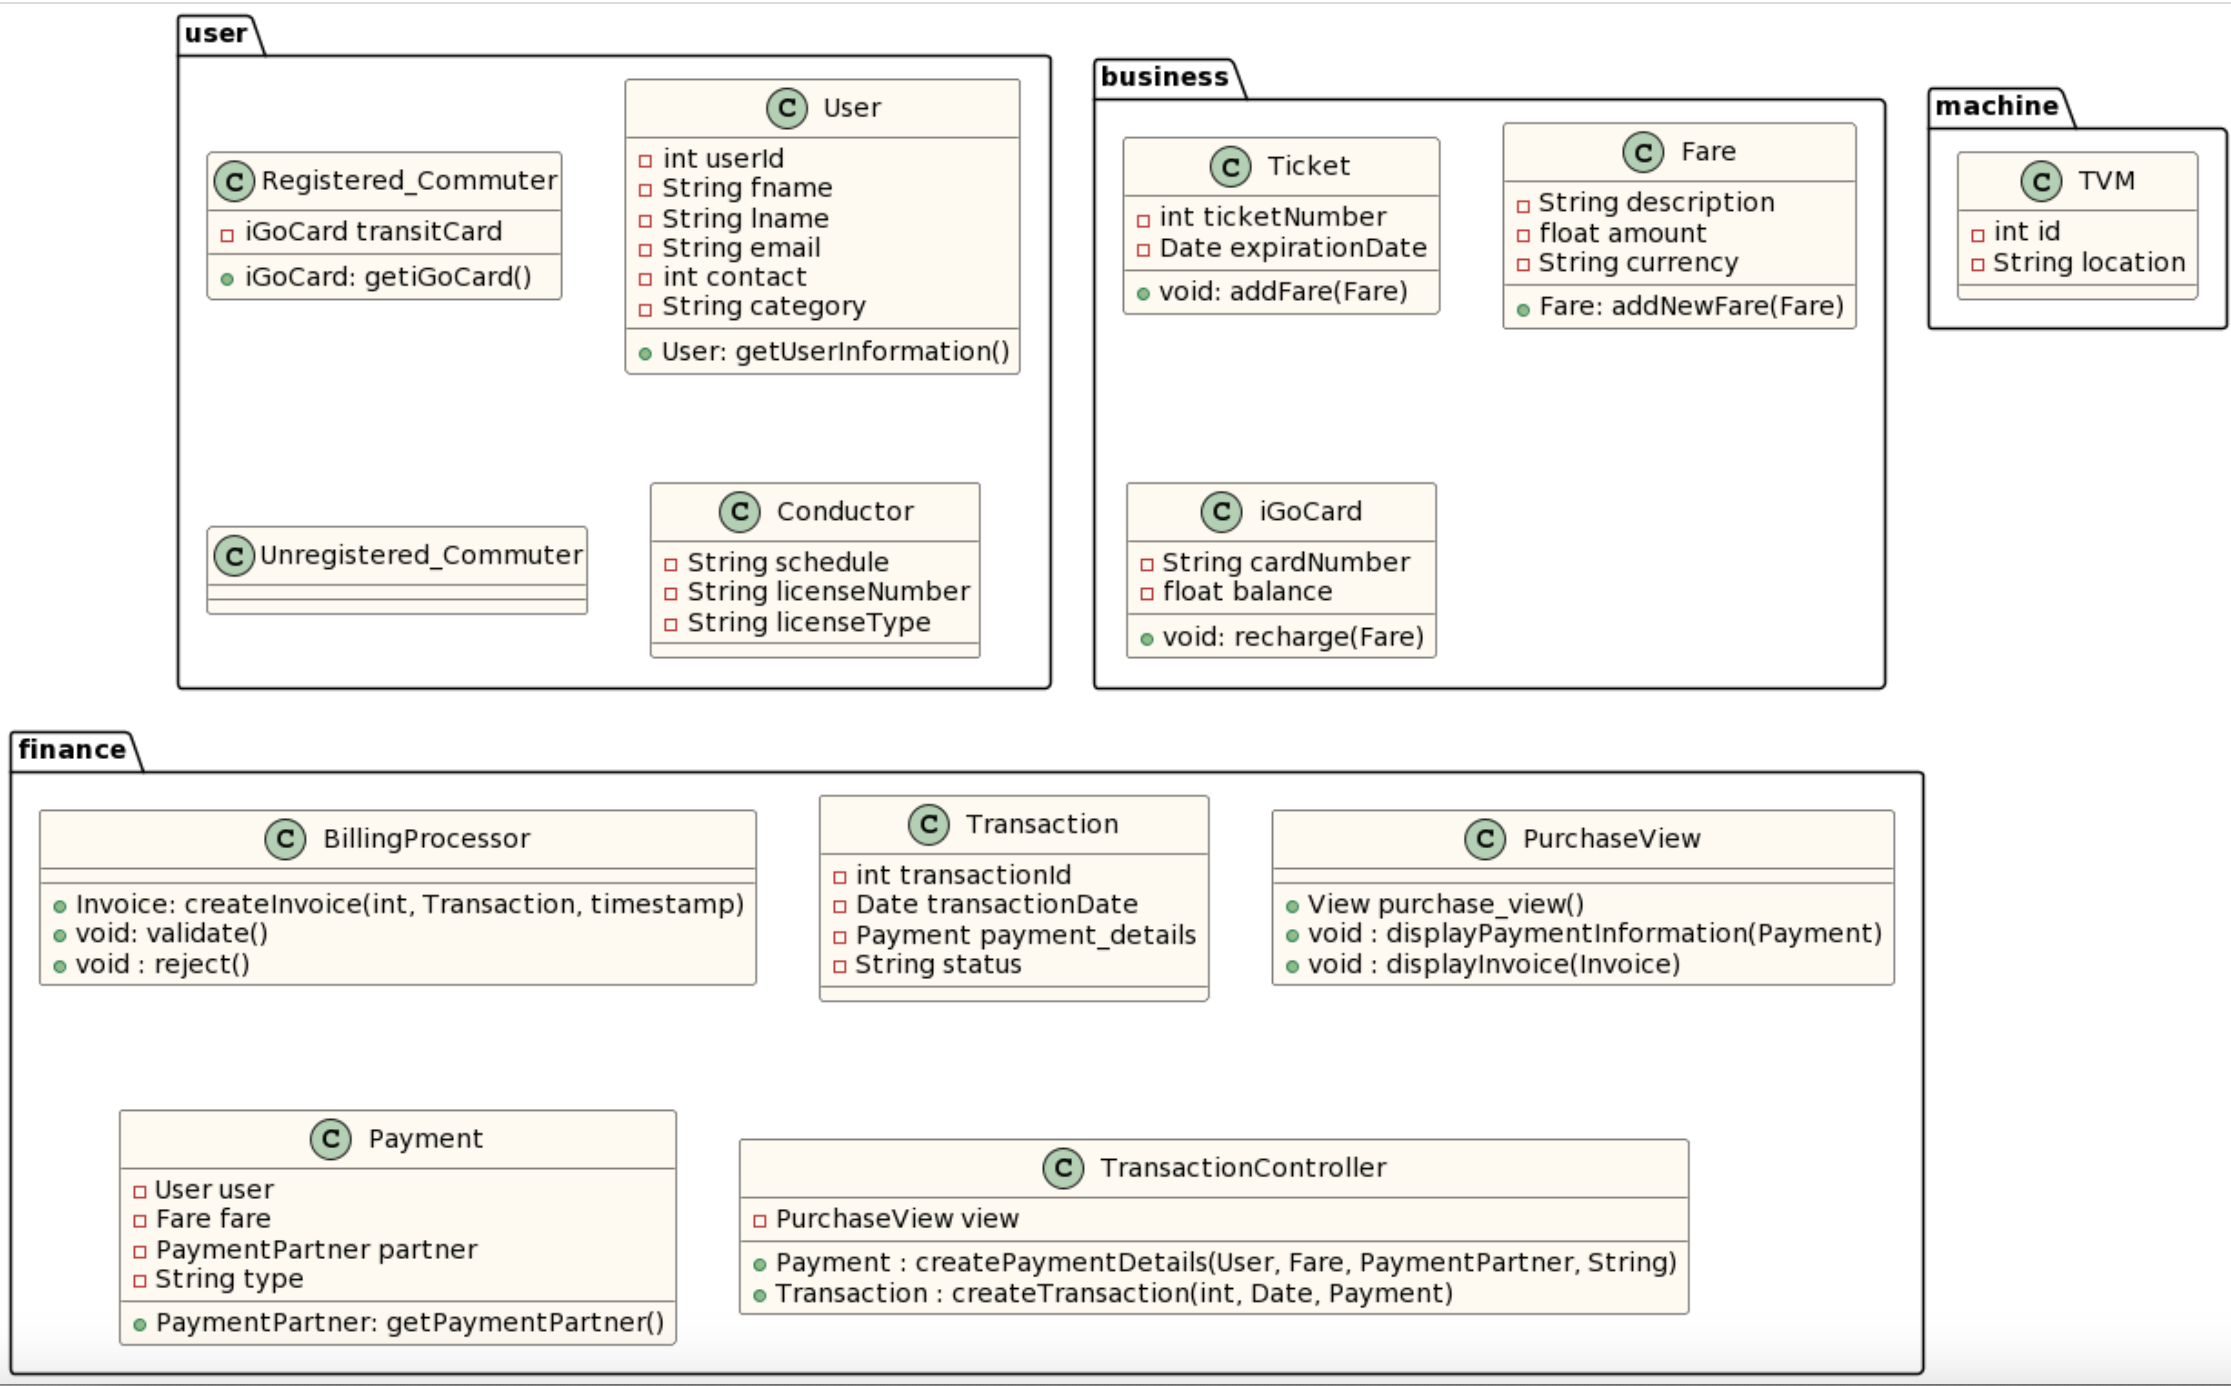
\includegraphics[width=150mm,height=130mm,scale=0.5]{D2-images/ClassDiagram.jpeg}
  \caption{iGO Class Diagram}
\end{figure}
\section{Low-level Solution Domain Model - Sequence Diagrams}
\subsection{iGO Sequence Diagram}
\begin{figure}[h!]
  \centering
   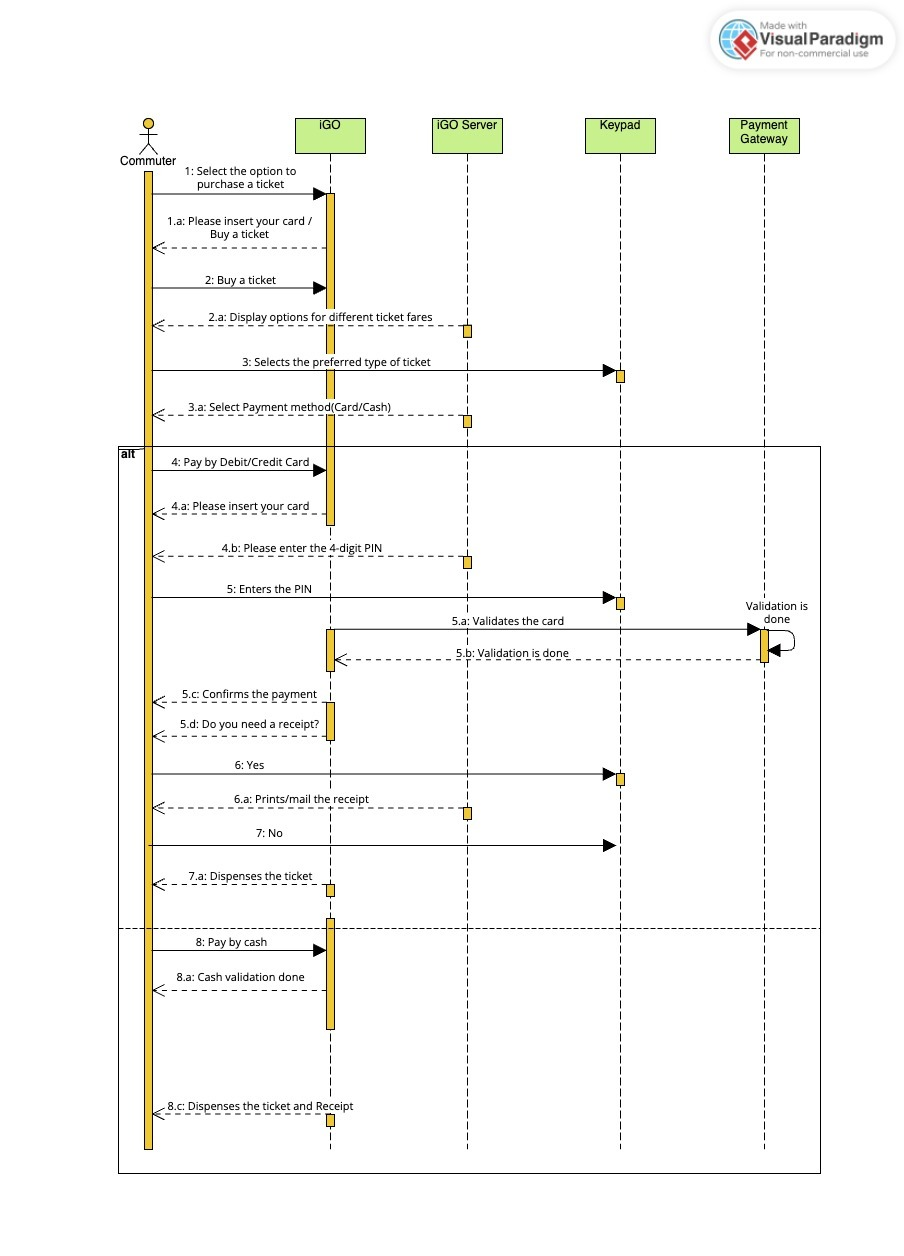
\includegraphics[width=150mm,height=200mm,scale=0.5]{D2-images/iGoSeq.jpg}
  \caption{iGO Sequence Diagram}
\end{figure}
\newpage
\subsection{Payment using card Sequence Diagram}
\begin{figure}[h!]
  \centering
   \includegraphics[width=150mm,height=130mm,scale=0.5]{D2-images/Payment_Sequence.png}
  \caption{Payment using card Sequence Diagram}
\end{figure}
\newpage
\subsection{Make Payment in Cash}
\begin{figure}[h!]
  \centering
   \includegraphics[width=150mm,height=180mm,scale=0.5]{D2-images/MakePaymentCash.jpeg}
  \caption{Payment in cash Sequence Diagram}
\end{figure}
\newpage
\subsection{Recharge Card}
\begin{figure}[h!]
  \centering
   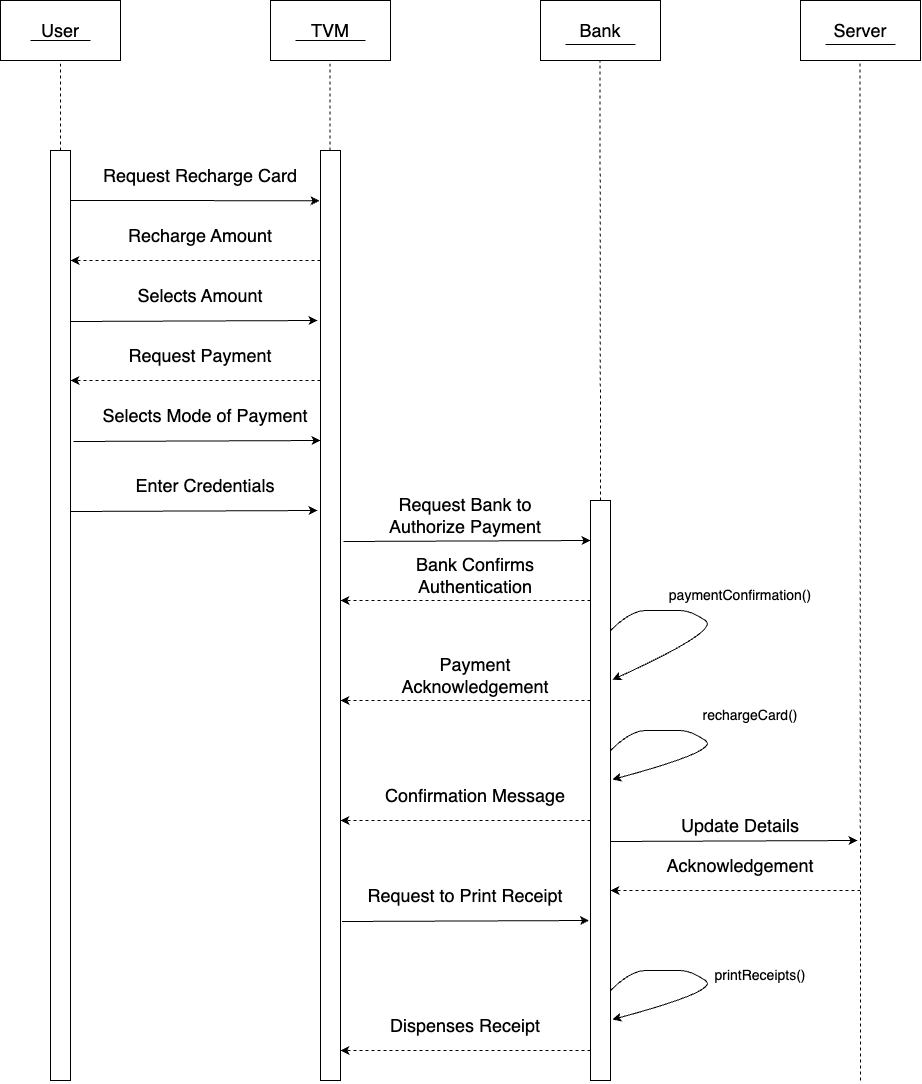
\includegraphics[width=150mm,height=130mm,scale=0.5]{D2-images/Sequence_diagram_recharge_card.png}
  \caption{Recharge Card Sequence Diagram}
\end{figure}
\newpage
\subsection{Recharge Card}
\begin{figure}[h!]
  \centering
   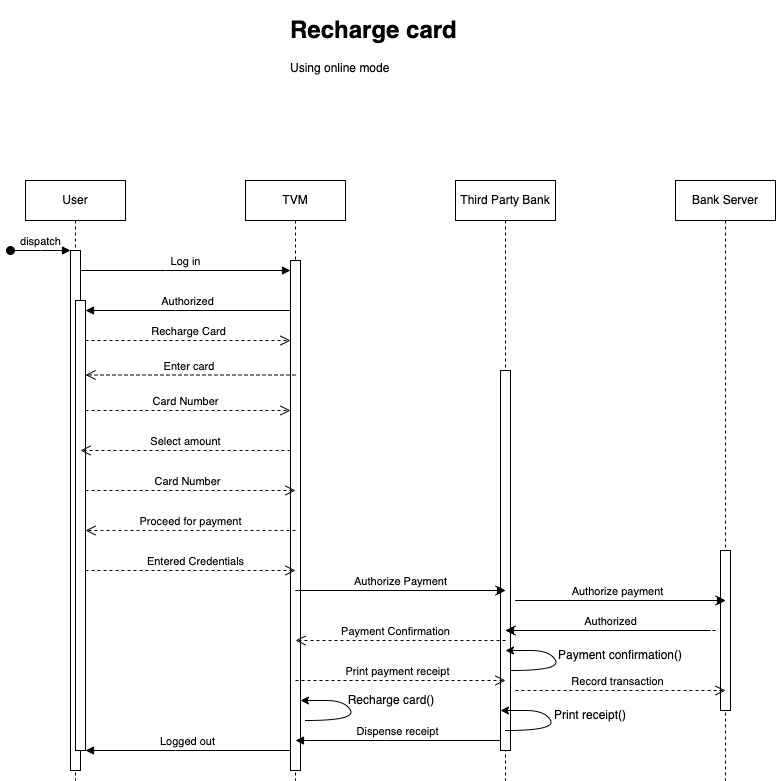
\includegraphics[width=150mm,height=180mm,scale=0.5]{D2-images/RechargeCardOnline.jpg}
  \caption{Recharge Card Using Online mode Sequence Diagram}
\end{figure}
\newpage
\subsection{Purchase Ticket}
\begin{figure}[h!]
  \centering
   \includegraphics[width=150mm,height=180mm,scale=0.5]{D2-images/PurchaseTicket.jpeg}
  \caption{Purchase Ticket Sequence Diagram}
\end{figure}

\chapter{Problem 8}
\asection{1}{Python Code}
\definecolor{codegreen}{rgb}{0,0.6,0}
\definecolor{codegray}{rgb}{0.5,0.5,0.5}
\definecolor{codepurple}{rgb}{0.58,0,0.82}
\definecolor{backcolour}{rgb}{0.95,0.95,0.92}

\lstdefinestyle{mystyle}{
    backgroundcolor=\color{backcolour},   
    commentstyle=\color{codegreen},
    keywordstyle=\color{magenta},
    numberstyle=\tiny\color{codegray},
    stringstyle=\color{codepurple},
    basicstyle=\ttfamily\footnotesize,
    breakatwhitespace=false,         
    breaklines=true,                 
    captionpos=b,                    
    keepspaces=true,                 
    numbers=left,                    
    numbersep=5pt,                  
    showspaces=false,                
    showstringspaces=false,
    showtabs=false,                  
    tabsize=2
}
\lstset{style=mystyle}
\begin{enumerate}
\item	In iGo implementation user can be of two types one is Child or Senior Citizens and another one is adult based on types of user fare will be decided. For demonstration purpose we gave access of iGo system to two types of users which are adult and child. 

\item \textbf{Select Language screen:} This is the first screen a user will see as soon as all things go as per the requirement of the iGo system, then the user will have two options in front of them which are English and French "Language options", Since a large group of English and French-speaking people are expected to be the potential users. two languages(English and French) are displayed to choose between:\\
\begin{lstlisting}[language=Python]
def select_language_display(username):
    print("Display Select Langauge:"+username)
    root.img = PhotoImage(file='login.png')
    Label(root,image=img,bg='white').place(x=50,y=50)
    frame = Frame(root,width=350,height=350,bg="white")
    frame.place(x=480,y=70)
    heading = Label(frame, text='Select Language', fg='#57a1f8',bg='white',font=('Microsoft YaHei UI Light',23,'bold'))
    heading.place(x=80,y=5)
    Button(frame,width=25,pady=7,text="English",bg='#ff8c00',fg='#57a1f8',font=('Microsoft YaHei UI Light',15,'bold','italic'),border=0,highlightbackground="#ff8c00",command=lambda: English_Language(username)).place(x=25,y=107)
    Button(frame,width=25,pady=7,text="French",bg='#ff8c00',fg='#57a1f8',font=('Microsoft YaHei UI Light',15,'bold','italic'),border=0,highlightbackground="#ff8c00",command=lambda: French_Language(username)).place(x=30,y=170)
\end{lstlisting}
\item \textbf{iGO Menu:}After selecting English or French user will have two options which are Recharge card and Buy Ticket.\\\\
After selecting Recharge Card or Buy Ticket user will have a set of options in iGo. These are Monthly Passes, Weekly Passes, Day Pass/Ticket, Weekend Pass, and One-way tickets. If the user will select French, then all options from now onwards will be in French only.\\\\

\begin{lstlisting}[language=Python]
def Select_Plans(username):
    print("Display Select Plans:"+username)
    root.img = PhotoImage(file='login.png')
    Label(root,image=img,bg='white').place(x=50,y=50)
    frame = Frame(root,width=400,height=550,bg="white")
    frame.place(x=450,y=70)
    heading = Label(frame, text='Select Language', fg='#57a1f8',bg='white',font=('Microsoft YaHei UI Light',23,'bold'))
    heading.place(x=70,y=5)
    Button(frame,width=25,pady=7,text="Monthly Pass",bg='#ff8c00',fg='#57a1f8',font=('Microsoft YaHei UI Light',15,'bold','italic'),border=0,highlightbackground="#ff8c00",command=lambda: Monthly_pass(username)).place(x=25,y=107)
    Button(frame,width=25,pady=7,text="Weekly Pass",bg='#ff8c00',fg='#57a1f8',font=('Microsoft YaHei UI Light',15,'bold','italic'),border=0,highlightbackground="#ff8c00",command=lambda: Weekly_pass(username)).place(x=30,y=170)
    Button(frame,width=25,pady=7,text="Day Pass",bg='#ff8c00',fg='#57a1f8',font=('Microsoft YaHei UI Light',15,'bold','italic'),border=0,highlightbackground="#ff8c00",command=lambda: Day_pass(username)).place(x=35,y=233)
    Button(frame,width=25,pady=7,text="Weekend Pass",bg='#ff8c00',fg='#57a1f8',font=('Microsoft YaHei UI Light',15,'bold','italic'),border=0,highlightbackground="#ff8c00",command=lambda: Weekend_pass(username)).place(x=40,y=296)
    Button(frame,width=25,pady=7,text="One Way Ticket",bg='#ff8c00',fg='#57a1f8',font=('Microsoft YaHei UI Light',15,'bold','italic'),border=0,highlightbackground="#ff8c00",command=lambda: One_way_pass(username)).place(x=45,y=359)
\end{lstlisting}
- After clicking on any of the above options user will have specific iGo layout based on the option which user is selecting. Apart from, Day Pass/Ticket and One way Ticket option user will have button of make payment directly with the price which user needs to pay for selecting any of the options from Monthly, Weekly or Weekend individually as per user’s selection. But when it comes to Day Pass/Ticket and one  One way ticket then user needs to enter no of tickets or pass which he needs. So, here it’s possible that user might enter nothing and try to press button named “Procced for Payment” in this case user will have popup showing message called “invalid input”. If user click “ok” button which will be there in popup then user will be redirected to selection options display where user will have again all the option which has been discussed earlier. Here we have handled exception as well so iGo might not get crashed.\\
\item \textbf{Monthly Pass:} The below method will display the details of the monthly pass:\\
\begin{lstlisting}[language=Python]
def Monthly_pass(username):
    print("Display Monthly Pass:"+username)
    root.img = PhotoImage(file='login.png')
    Label(root,image=img,bg='white').place(x=50,y=50)
    frame = Frame(root,width=400,height=550,bg="white")
    frame.place(x=480,y=70)
    heading = Label(frame, text='Monthly Pass', fg='#57a1f8',bg='white',font=('Microsoft YaHei UI Light',23,'bold'))
    heading.place(x=100,y=5)
    if username == 'child' or username == 'senior citizens':
        button = Button(frame,width=25,pady=7,text="Make Payment: $50",bg='#ff8c00',fg='#57a1f8',font=('Microsoft YaHei UI Light',15,'bold','italic'),border=0,highlightbackground="#ff8c00",command=lambda: select_payment_option(username)).place(x=35,y=120)
    else:
        button = Button(frame,width=25,pady=7,text="Make Payment: $60",bg='#ff8c00',fg='#57a1f8',font=('Microsoft YaHei UI Light',15,'bold','italic'),border=0,highlightbackground="#ff8c00",command=lambda: select_payment_option(username)).place(x=35,y=120)
\end{lstlisting}
\item \textbf{Weekly Pass:} The below method will display the details of the weekly pass:\\
\begin{lstlisting}[language=Python]
def Weekly_pass(username):
    print("Display Weekly Pass:"+username)
    root.img = PhotoImage(file='login.png')
    Label(root,image=img,bg='white').place(x=50,y=50)
    frame = Frame(root,width=400,height=550,bg="white")
    frame.place(x=440,y=70)
    heading = Label(frame, text='Weekly Pass', fg='#57a1f8',bg='white',font=('Microsoft YaHei UI Light',23,'bold'))
    heading.place(x=100,y=5)
    if username == 'child' or username == 'senior citizens':
        button = Button(frame,width=25,pady=7,text="Make Payment: $10",bg='#ff8c00',fg='#57a1f8',font=('Microsoft YaHei UI Light',15,'bold','italic'),border=0,highlightbackground="#ff8c00",command=lambda: select_payment_option(username)).place(x=35,y=120)
    else:
        button = Button(frame,width=25,pady=7,text="Make Payment: $15",bg='#ff8c00',fg='#57a1f8',font=('Microsoft YaHei UI Light',15,'bold','italic'),border=0,highlightbackground="#ff8c00",command=lambda: select_payment_option(username)).place(x=35,y=120)
\end{lstlisting}
\item \textbf{Day Pass:} The below method will display the details of the Day pass:\\
\begin{lstlisting}[language=Python]
def Day_pass(username):    
    print("Display Day Pass:"+username)
    root.img = PhotoImage(file='login.png')
    Label(root,image=img,bg='white').place(x=50,y=50)
    frame = Frame(root,width=400,height=550,bg="white")
    frame.place(x=480,y=70)
    heading = Label(frame, text='Day Pass', fg='#57a1f8',bg='white',font=('Microsoft YaHei UI Light',23,'bold'))
    heading.place(x=100,y=5)
    No_ticket = Label(frame, text = "No. of Tickets",fg="#57a1f8",font=('Microsoft YaHei UI Light',15,'bold'))
    No_ticket.place(x = 30,y = 70)
    tickets = Entry(frame, width=25,fg='black',border=0,bg="white",font=('Microsoft YaHei UI Light',11))
    tickets.place(x=150,y=73)
    tickets.insert(0,'')
    tickets.bind('<FocusIn>',on_enter)
    tickets.bind('<FocusOut>',on_leave)
    Frame(frame,width=200,height=1.5,bg='black').place(x=140,y=100)
    button = Button(frame,width=25,pady=7,text="Proceed For Payment",bg='#ff8c00',fg='#57a1f8',font=('Microsoft YaHei UI Light',15,'bold','italic'),border=0,highlightbackground="#ff8c00",command=lambda: tickets_calculation(tickets,username)).place(x=35,y=120)
\end{lstlisting}
\item \textbf{Weekend Pass:} The below method will display the details of the Weekend pass\\
\begin{lstlisting}[language=Python]
def Weekend_pass(username):
    print("Display Weekend Pass:"+username)
    root.img = PhotoImage(file='login.png')
    Label(root,image=img,bg='white').place(x=50,y=50)
    frame = Frame(root,width=400,height=550,bg="white")
    frame.place(x=440,y=70)
    heading = Label(frame, text='Weekend Pass', fg='#57a1f8',bg='white',font=('Microsoft YaHei UI Light',23,'bold'))
    heading.place(x=100,y=5)    
    if username == 'child' or username == 'senior citizens':
        button = Button(frame,width=25,pady=7,text="Make Payment: $4",bg='#ff8c00',fg='#57a1f8',font=('Microsoft YaHei UI Light',15,'bold','italic'),border=0,highlightbackground="#ff8c00",command=lambda: select_payment_option(username)).place(x=35,y=120)
    else:
        button = Button(frame,width=25,pady=7,text="Make Payment: $5",bg='#ff8c00',fg='#57a1f8',font=('Microsoft YaHei UI Light',15,'bold','italic'),border=0,highlightbackground="#ff8c00",command=lambda: select_payment_option(username)).place(x=35,y=120)
\end{lstlisting}
\item \textbf{One Way Ticket:} The below method will display the details of one-way ticket:\\
\begin{lstlisting}[language=Python]
def One_way_pass(username):
    print("Display One Day Pass:"+username)
    root.img = PhotoImage(file='login.png')
    Label(root,image=img,bg='white').place(x=50,y=50)
    frame = Frame(root,width=400,height=550,bg="white")
    frame.place(x=480,y=70)
    heading = Label(frame, text='One way Pass', fg='#57a1f8',bg='white',font=('Microsoft YaHei UI Light',23,'bold'))
    heading.place(x=100,y=5)
    No_ticket = Label(frame, text = "No. of Tickets",fg="#57a1f8",font=('Microsoft YaHei UI Light',15,'bold'))
    No_ticket.place(x = 30,y = 70)
    tickets = Entry(frame, width=25,fg='black',border=0,bg="white",font=('Microsoft YaHei UI Light',11))
    tickets.place(x=150,y=73)
    tickets.insert(0,'')
    tickets.bind('<FocusIn>',on_enter)
    tickets.bind('<FocusOut>',on_leave)
    Frame(frame,width=200,height=1.5,bg='black').place(x=140,y=100)
    button = Button(frame,width=25,pady=7,text="Proceed For Payment",bg='#ff8c00',fg='#57a1f8',font=('Microsoft YaHei UI Light',15,'bold','italic'),border=0,highlightbackground="#ff8c00",command=lambda: tickets_calculation(tickets,username)).place(x=35,y=120)
\end{lstlisting}
-	For the two options which are Day Pass/Ticket and One way ticket if user enter correct input and for the rest of the other option after selecting “Make Payment button user will have two options which are “Payment Options” named as “Credit card/ Debit card” and “Cash \\
\item \textbf{Checkout screen:} The below methods will calculate the price for the selected tickets/pass and then display on the screen\\
\begin{lstlisting}[language=Python]
def tickets_calculation(tickets,username):
    print("Monthly Plan:"+username)
    no_tickets = tickets.get()
    root.img = PhotoImage(file='login.png')
    Label(root,image=img,bg='white').place(x=50,y=50)
    frame = Frame(root,width=400,height=550,bg="white")
    frame.place(x=480,y=70)    
    if username == 'child' or username == 'senior citizens':
        total_cost = float(no_tickets) * 1.99
        print(total_cost)
        button = Button(frame,width=25,pady=7,text="Make Payment of "+str(total_cost),bg='#ff8c00',fg='#57a1f8',font=('Microsoft YaHei UI Light',15,'bold','italic'),border=0,highlightbackground="#ff8c00",command=lambda: select_payment_option(username)).place(x=35,y=120)
    else:
        total_cost = float(no_tickets) * 2.99
        button = Button(frame,width=25,pady=7,text="Make Payment of "+str(total_cost),bg='#ff8c00',fg='#57a1f8',font=('Microsoft YaHei UI Light',15,'bold','italic'),border=0,highlightbackground="#ff8c00",command=lambda: select_payment_option(username)).place(x=35,y=120)
        print(total_cost)
\end{lstlisting}
\item \textbf{Payment Options:} The below method will ask user to select debit/credit or Cash for payment\\
\begin{lstlisting}[language=Python]
def creditdebit(username):
    print("Display Credit Debit Option:"+username)
    root.img = PhotoImage(file='login.png')
    Label(root,image=img,bg='white').place(x=50,y=50)
    frame = Frame(root,width=400,height=550,bg="white")
    frame.place(x=440,y=70)
    heading = Label(frame, text='Almost Done!!!!!', fg='#57a1f8',bg='white',font=('Microsoft YaHei UI Light',23,'bold'))
    heading.place(x=100,y=5)
    messagebox.showinfo("Payment Processing", "Payment is being processed...")
    # Insert code here to process the payment, e.g. call an API or perform necessary actions
    messagebox.showinfo("Payment Success", "Payment has been successfully processed!")
    Button(frame,width=25,pady=7,text="Print Invoice",bg='#ff8c00',fg='#57a1f8',font=('Microsoft YaHei UI Light',15,'bold','italic'),border=0,highlightbackground="#ff8c00",command=lambda: printinvoice(username)).place(x=40,y=107)
\end{lstlisting}
\item \textbf{Select payment screen:} The below method will display the payment screen\\\\
-	After selecting “Credit card/ Debit card” option user must enter his Debit/Credit card number. Here, if user will enter nothing and press “Proceed for Payment” then user will get popup like “invalid Input”. Here, we handled the exception. So, if user enter incorrect card number, then system needs to stop user to make payment. So, we have been considered security concerns for payment as well.  After entering correct card number user will get two popups like “Payment is being processed...” and after that “Payment has been successfully processed!”. At the end user can also print invoice by clicking on “Print Invoice” button.\\\\
\begin{lstlisting}[language=Python]
def select_payment_option(username):
    print("Display Payment Option:"+username)
    root.img = PhotoImage(file='login.png')
    Label(root,image=img,bg='white').place(x=50,y=50)
    frame = Frame(root,width=400,height=550,bg="white")
    frame.place(x=440,y=70)
    heading = Label(frame, text='Payment Options', fg='#57a1f8',bg='white',font=('Microsoft YaHei UI Light',23,'bold'))
    heading.place(x=100,y=5)
    Button(frame,width=25,pady=7,text="Credit/Debit Card",bg='#ff8c00',fg='#57a1f8',font=('Microsoft YaHei UI Light',15,'bold','italic'),border=0,highlightbackground="#ff8c00",command=lambda: creditdebit(username)).place(x=40,y=107)
    Button(frame,width=25,pady=7,text="Cash",bg='#ff8c00',fg='#57a1f8',font=('Microsoft YaHei UI Light',15,'bold','italic'),border=0,highlightbackground="#ff8c00").place(x=40,y=170)
\end{lstlisting}
\item \textbf{Print Invoice}: The below method will print the Invoice of the ticket after the successful payment by the user\\
\begin{lstlisting}[language=Python]
def printinvoice(username):
    print("Display Print Invoice Option:"+username)
    messagebox.showinfo("Printing Your Invoice", "Printing is under process!!")
    # Insert code here to process the payment, e.g. call an API or perform necessary actions
    messagebox.showinfo("Printing Done", "Printing has been successfully completed!")
\end{lstlisting}
\end{enumerate}
\newpage
\asection{2}{Exception Handling}
\begin{enumerate}
    \item -	We handled several exceptions as well and kept several validations throughout the iGo system for security purpose. So, if user tries to press Login button without entering id which is “child or adult” in this case and password is “1234” then iGo will handle this exception by showing popup message which is “invalid username and password” or “invalid username” or “invalid password” based on the credentials enter by user.\\
\end{enumerate}
\begin{lstlisting}[language=Python]
def signin():
    username = user.get()
    password_input = password.get()
#     child
    if username == 'child' and password_input == '1234':
#         Select Language
        select_language_display(username)
    elif username == 'adult' and password_input == '1234':
        select_language_display(username)
    elif (username != 'child' or username != 'adult') and password_input != '1234': 
        messagebox.showerror("Invalid","invalid username and password")
    elif password_input != '1234': 
        messagebox.showerror("Invalid","invalid password")
    elif username != 'child': 
        messagebox.showerror("Invalid","invalid username") 
    elif username != 'adult': 
        messagebox.showerror("Invalid","invalid username") 
\end{lstlisting}
\begin{figure}[h!]
  \centering
   \includegraphics[width=100mm,height=70mm,scale=0.5]{D2-images/2.jpg}
  \caption{Validation for Username and Password}
\end{figure}
\begin{figure}[h!]
  \centering
   \includegraphics[width=100mm,height=70mm,scale=0.5]{D2-images/err2.jpg}
  \caption{Debit/Credit Card Validation screen}
\end{figure}
\begin{figure}[h!]
  \centering
   \includegraphics[width=100mm,height=70mm,scale=0.5]{D2-images/err4.jpg}
  \caption{User Input Validation}
\end{figure}
\chapter{Problem 9}
\asection{1}{Screenshots}
\begin{figure}[h!]
  \centering
   \includegraphics[width=100mm,height=70mm,scale=0.5]{D2-images/2.jpg}
  \caption{Main Page of the Application}
\end{figure}

\begin{figure}[h!]
  \centering
   \includegraphics[width=100mm,height=70mm,scale=0.5]{D2-images/3.jpg}
  \caption{Language Selection screen}
\end{figure}

\begin{figure}[h!]
  \centering
   \includegraphics[width=100mm,height=70mm,scale=0.5]{D2-images/4.jpg}
  \caption{iGo - Menu screen}
\end{figure}

\begin{figure}[h!]
  \centering
   \includegraphics[width=100mm,height=70mm,scale=0.5]{D2-images/5.jpg}
  \caption{iGO - User Pass Selection screen}
\end{figure}

\begin{figure}[h!]
  \centering
   \includegraphics[width=100mm,height=70mm,scale=0.5]{D2-images/6.jpg}
  \caption{iGO - Monthly Pass Checkout screen}
\end{figure}

\begin{figure}[h!]
  \centering
   \includegraphics[width=100mm,height=70mm,scale=0.5]{D2-images/7.jpg}
  \caption{iGO - Payment screen}
\end{figure}

\begin{figure}[h!]
  \centering
   \includegraphics[width=100mm,height=70mm,scale=0.5]{D2-images/8.jpg}
  \caption{iGO - Payment Processing screen}
\end{figure}

\begin{figure}[h!]
  \centering
   \includegraphics[width=100mm,height=70mm,scale=0.5]{D2-images/9.jpg}
  \caption{iGO - Payment Successful screen}
\end{figure}

\begin{figure}[h!]
  \centering
   \includegraphics[width=100mm,height=70mm,scale=0.5]{D2-images/10.jpg}
  \caption{iGO - Print Invoice Screen}
\end{figure}

\begin{figure}[h!]
  \centering
   \includegraphics[width=100mm,height=70mm,scale=0.5]{D2-images/11.jpg}
  \caption{iGO - Print Successful screen}
\end{figure}

\begin{figure}[h!]
  \centering
   \includegraphics[width=100mm,height=70mm,scale=0.5]{D2-images/12.jpg}
  \caption{iGO - Weekly Pass Checkout screen}
\end{figure}

\begin{figure}[h!]
  \centering
   \includegraphics[width=100mm,height=70mm,scale=0.5]{D2-images/13.jpg}
  \caption{iGO - Day Pass Checkout screen}
\end{figure}

\begin{figure}[h!]
  \centering
   \includegraphics[width=100mm,height=70mm,scale=0.5]{D2-images/14.jpg}
  \caption{iGO - Day Pass Payment screen}
\end{figure}

\begin{figure}[h!]
  \centering
   \includegraphics[width=100mm,height=70mm,scale=0.5]{D2-images/15.jpg}
  \caption{iGO - Weekend Pass Checkout screen}
\end{figure}


\begin{figure}[h!]
  \centering
   \includegraphics[width=100mm,height=70mm,scale=0.5]{D2-images/16.jpg}
  \caption{iGO - One-way Ticket Checkout screen}
\end{figure}

\begin{figure}[h!]
  \centering
   \includegraphics[width=100mm,height=70mm,scale=0.5]{D2-images/17.jpg}
  \caption{iGo - French Version}
\end{figure}


\chapter{References}
\begin{enumerate}
  \item \url{http://www.stm.info/en}
  \item PANKAJ KAMTHAN (2023) “Understanding Context"
  \item PANKAJ KAMTHAN (2023) “Introduction to Interviews”
  \item PANKAJ KAMTHAN (2023) “Introduction To Domain Modeling” - Section 14, 15 ,16.
  \item PANKAJ KAMTHAN (2023) “Introduction To Use Case Modeling” - Section 11, 12.
  \item PANKAJ KAMTHAN (2023) “Negative Use Case Modeling”  - Section 8
  \item \url{https://www.lucidchart.com/pages/uml-activity-diagram}
  \item Carte OPUS. To obtain your photo OPUS card. 2023. \url{http://www.carteopus.info/}.
  \item Code Formatting in LaTeX \url{https://www.overleaf.com/learn/latex/Code_listing}
\end{enumerate}
\end{document}